\documentclass[a4paper,12pt]{article}

\usepackage[left=1in, right=1in, top=0.5in, bottom=1in]{geometry}
\usepackage[latin2]{inputenc} 
\usepackage{amsmath}
\usepackage{graphicx} 
\usepackage[T1]{fontenc} 
\usepackage{color}
\usepackage{amssymb} 
\usepackage{times}
\usepackage{subfig}

\newcommand{\lhood}{\ensuremath{\mathcal{L}}}
\newcommand{\truth}{\ensuremath{\mathcal{T}}}
\newcommand{\model}{\ensuremath{\mathcal{M}}}
\newcommand{\optmodel}{\ensuremath{\mathcal{M}^*}}

\DeclareMathOperator*{\argmin}{arg\,min}
\DeclareMathOperator*{\argmax}{arg\,max}

% Some useful macros

\definecolor{Cgreen}{rgb}{0,0.6,0}
\definecolor{Cblue}{rgb}{0,0.39,0.61}

\newcounter{ohNoteCounter} \newcommand{\ohnote}[1]{{\scriptsize
    \color{Cgreen}
    $\clubsuit$~\refstepcounter{ohNoteCounter}\textsf{[OH]$_{\arabic{ohNoteCounter}}$:{#1}}}}

\newcounter{jpNoteCounter} \newcommand{\jpnote}[1]{{\scriptsize
    \color{Cblue} $\blacksquare$
    \refstepcounter{jpNoteCounter}\textsf{[JP]$_{\arabic{jpNoteCounter}}$:{#1}}}}

\IfFileExists{.notes_disabled}{ \renewcommand{\jpnote}[1]{}
  \renewcommand{\ohnote}[1]{} }

\title { \normalsize Graphical Markov Models \\ Winter 2011 \\
 \vspace{10mm} {\bf Identifying License Plates Ids with Hidden Markov
    Models } }
\author{\normalsize James Pritts and Ondrej Hrstka }
\date{ \small January 2012 }

\begin{document}
\maketitle

\pagestyle{empty} 
\section*{1. DRAFT}
\section{Problem Statement}
The problem is to report the unique identifying string of characters,
called the \emph{vehicle-id}, of a license plate.  Provided are images
of license plates that have been segmented and ortho-rectified. A
subset of these images each have the following corresponding
annotations: a top and bottom boundary that delimits the
\emph{vehicle-id} within the segmented license plate, a bounding box
of each character and white-space interval that comprises the
\emph{vehicle-id}, and a character label for each bounding box that
contains a character.  We assume that the font of all characters
across license plates is identical, and we refer to a particular
character of the font set as a glyph.

\section{Preliminaries}
Let $I\colon \mathbb{Z}^2_+ \to \mathbb{R}$ be a function that maps a
point $\mathbf{u} = (i,j)$ to a real value $x_{ij}$, such that $I$
gives the raw intensity value at each point in the image.  Denote
$\mathbf{x}_i$ and $\mathbf{x}_j$ as the row and column of pixels in
the image at row $i$ and column $j$ respectively.

To condense the notation for probability distributions, we denote
$p_{x_{ij} \mid s_j}(x_{ij} \mid s_j)$ by writing $p(x_{ij} \mid
s_j)$; in other words, the arguments of $p$ will uniquely select the
proper density function for evaluation.

\section{Model Definition}
We model a \emph{vehicle-id} by a Hidden Markov Model (\textbf{HMM}).
The characters of the \emph{vehicle-id} are assumed to come from the
same font set, so any image of a particular character can be mapped to
the same glyph.  The left-to-right sequence of consecutive columns
from the segmented license plate are the \emph{observations}.

The set of \emph{hidden states} $\mathbf{K}$ are the column indexes of
all the glyphs in the font set and an added state $w$ that represents
white-space. An example sequence of hidden states $S \in \mathbf{K}^n$
is
\[S =
\left(\,\dots,\text{w},\text{A}_1,\text{A}_2,\ldots,\text{A}_{m},\text{w},\text{w},\text{w},\text{T}_1,\text{T}_2,\ldots\,\right).\]

The \emph{emission probabilities} are the probabilities of observing
pixel intensities given their corresponding glyph column, or,
equivalently, given their \emph{hidden states}. We make the
simplifying assumption that probabilities of observing intensities in
a column $\mathbf{x}_j$ are pairwise independent \[p(\mathbf{x}_j \mid
s_j) = \prod_{i=1}^np(x_{ij} \mid s_j).\] The probability of observing
pixel intensity $x_{ij}$ of a glyph column $s_j$ is modeled as a
two-class gaussian mixture, where the first class $c=f$ contains
foreground pixels, and the second class $c=b$ contains background
pixels,
\begin{align*}
  p(x_{ij} \mid s_j) &= p(x_{ij},c=f \mid s_j)+p(x_{ij},c=b \mid s_j)\\
  &= p(x_{ij}\mid c=f,s_j)p(c=f \mid s_j)+p(x_{ij} \mid c=b,s_j)p(c=b \mid s_j) \\
  &= p(x_{ij}\mid c=f)p(c=f \mid s_j)+p(x_{ij} \mid c=b)p(c=b \mid s_j) \\
  &= \mathcal{N}(\sigma_1,\mu_1)\gamma_{is_j}+\mathcal{N}(\sigma_2,\mu_2)(1-\gamma_{is_j}).
\end{align*}
The model for \emph{emissions probabilities} assumes that the
foreground and background distributions are position independent,
while the mixture parameter depends on the row position of the glyph
column $s_j$.

\begin{figure}[htp]
\centering
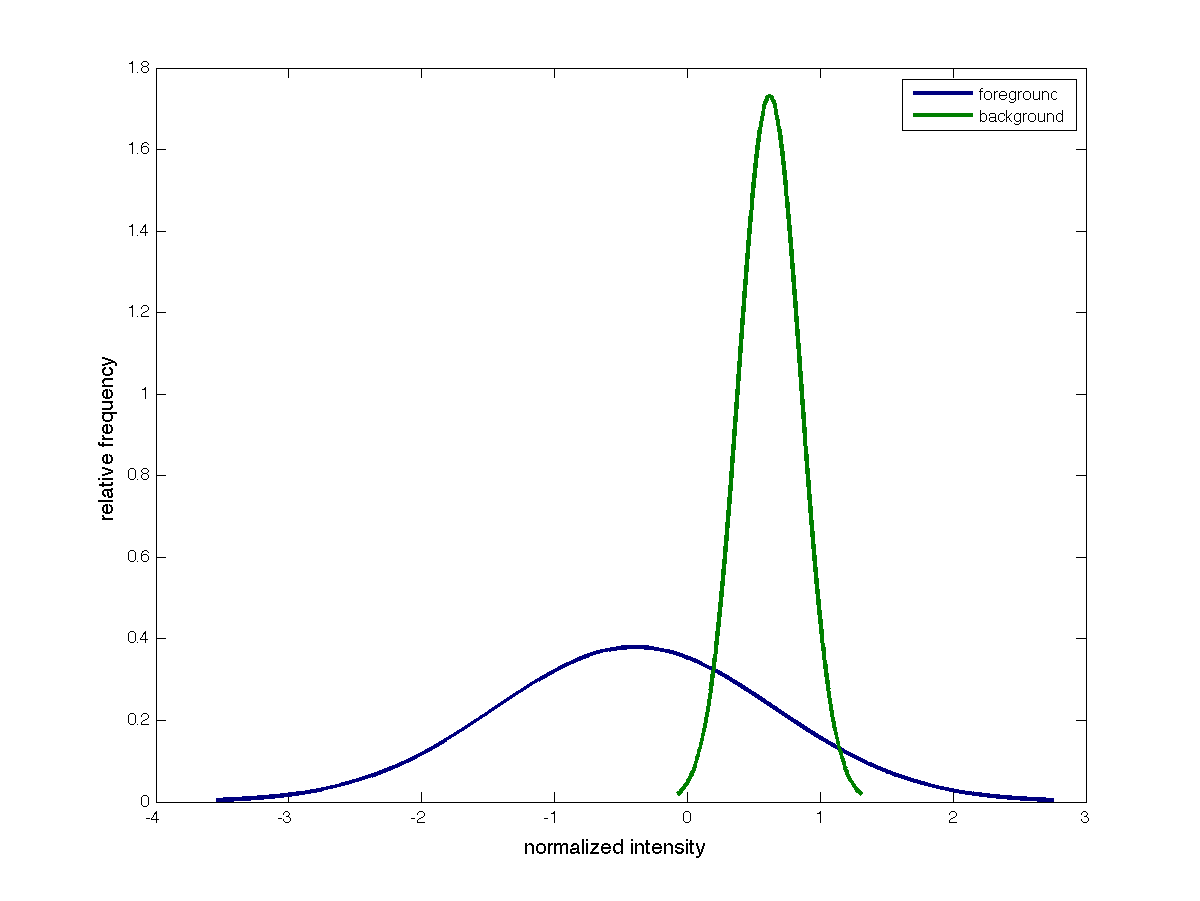
\includegraphics[width=\linewidth]{pics/distribution.png}
\caption{ Learned global foreground (in blue) $ p(x_{ij}\mid c=f,s_j)$ and
  background (in green) $p(x_{ij} \mid c=b,s_j)$ image intensity models }
\label{fig:distribution}
\end{figure}

\section{Learning the Emission Probabilities}
The annotated data $\truth$ does not contain segmentations of
vehicle-id characters from the background, rather the annotation are
loose bounding boxes that contain significant white-space. Thus,
\emph{Unsupervised learning} will be required to specify the
\emph{emissions probabilities} $p(x_{ij} \mid s_j)$.

Denote the set of parameters needed to determine the model of a glyph
column $j$ as
\[\model_{k_j}=\{\,\mu_1,\sigma_1,\mu_2,\sigma_2,\gamma_{1,k_j},\gamma_{2,k_j},\ldots,\gamma_{m,k_j}\,\}.\]
Then the model for all columns of all glyphs in the entire font set is
specified as
\[
\model = \cup_{i=1}^m\model_{k_i}.
\]

Given the annotated data $\truth$, we seek the maximum-likelihood
estimate \[ \optmodel = \argmax_{\model} \lhood(\truth \mid \model).\]

Regardless, varying character widths are not fully accounted for in
the \textbf{HMM}. As a fix, we chose to set the glyph template width
as the median of all exemplars of the glyph in the training
set. Models were learned from exemplars with median width. Exemplars with different width were filtered out.
\jpnote{Need explanation of how filtering was accomplished. How were
  emission probabilities calcuated with filtering}
\ohnote{This is short but sufficient I think}

Learning a model for a glyph column comprises of learning the
position-independent global foreground $ p(x_{ij}\mid
c=f,s_j)=\mathcal{N}(\sigma_1,\mu_1)$ and background $p(x_{ij} \mid
c=b,s_j)=\mathcal{N}(\sigma_2,\mu_2)$ image intensity models, as well
their position-dependent and glyph-dependent priors. Expectation
Maximization is to learn these parameters.

At E-step $t+1$ probability of each pixel $d$ from training dataset $d \in \mathcal{D}$ is calculated with respect to given model $\model^t$:
\[
  p(x_{ij} \mid c=f, s_j)_d^{t+1} = \frac{\mathcal{N}(\sigma_1^t,\mu_1^t)\gamma_{is_j}^t}{\mathcal{N}(\sigma_1^t,\mu_1^t)\gamma_{is_j}^t+\mathcal{N}(\sigma_2^t,\mu_2^t)(1-\gamma_{is_j}^t)}
\]

At M-step $i+1$ parameters of model $\model^{t+1}$ are maximized with respect to $p(x \mid c=f, s)^{t+1}$:
\[
  \gamma_{is_j}^{t+1} = \frac{\sum_{d \in \mathcal{D}} p(x_{ij} \mid c=f, s_j)_d^{t+1}}{\sum_{d \in \mathcal{D}} p(x_{ij} \mid c=f, s_j)_d^{t+1} + \sum_{d \in \mathcal{D}} (1-p(x_{ij} \mid c=b, s_j)_d^{t+1})}
\]
\[
  \sigma_1^{t+1} = \frac{\sum_{i,j} \sum_{d \in \mathcal{D}} x_{d, i,j} p(x_{ij} \mid c=f, s_j)_d^{t+1} }{\sum_{i,j} \sum_{d \in \mathcal{D}} p(x_{ij} \mid c=f, s_j)_d^{t+1}}
\]
The parameters $\sigma_2^{t+1}, \mu_1^{t+1}, \mu_2^{t+1}$ are calculated in similar way.

The algorithm is stopped when condition $|1-\frac{\sigma_1^{t+1}}{\sigma_1^{t}}| < \epsilon \wedge |1-\frac{\sigma_2^{t+1}}{\sigma_2^{t}}| < \epsilon$ holds, where $\epsilon$ has been set to value $10^{-5}$.
\jpnote{Need equations for expectation step and maximization step.}


\begin{figure}[htp]
\centering
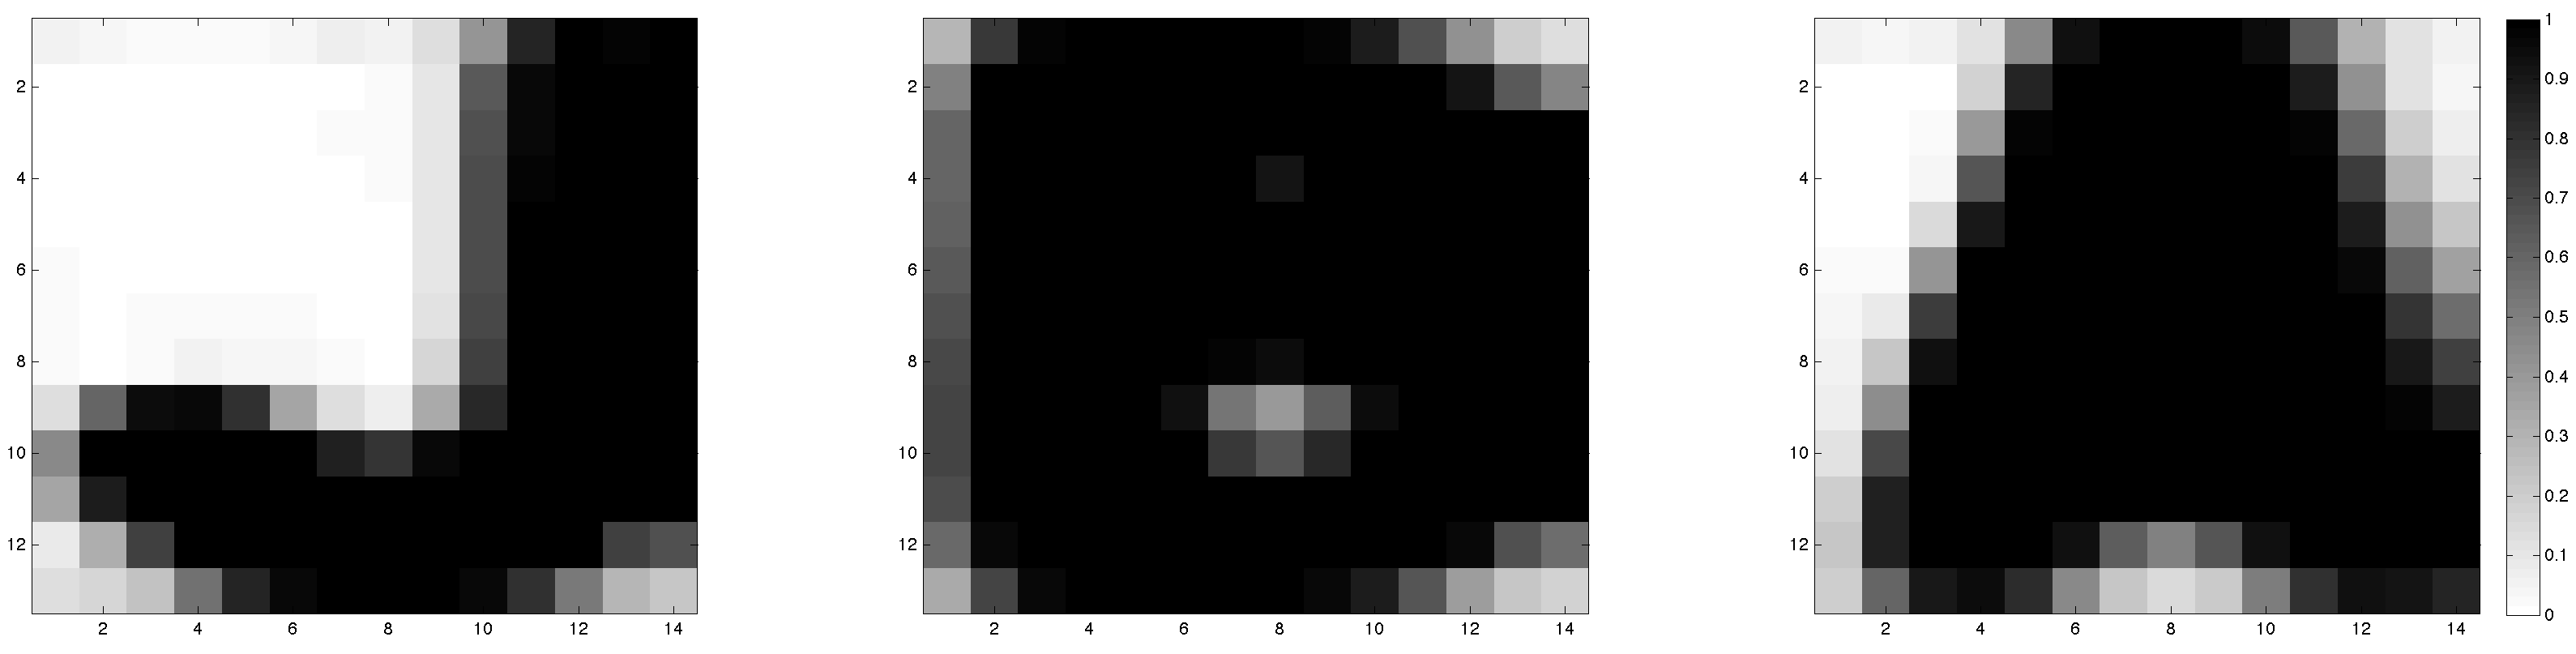
\includegraphics[width=\linewidth]{pics/jba.png}
\caption{Learned templates of \texttt{J}, \texttt{B} and
  \texttt{A}. Intensity corresponds to the prior probability for being
  a foreground pixel.}
\label{fig:templates}
\end{figure}

\section{Setting the Transition Probabilities}
Permitted transitions were set by hand based on some qualitative
observations of the given license-plate data. Allowed transitions
include white-space to white-space, white-space to first glyph
columns, between consecutive glyph columns, between terminal glyph
columns and white-space. Additionally, to allow for variance in
character widths, we allow transitions to the same glyph
column. Transitions to non-consecutive glyph columns and from
non-terminal glyph columns to white-space are prohibited.

Transition probabilities were also derived qualitatively from the
data. For example, the expected value of the length of consecutive
white-space characters was used to compute the probability of
white-space to white-space transition.

\section{Inference}
The hamming loss function is used for inference.  To find the most
probable sequence $s$, the probabilities $p(x,s_i)$ are first computed
by multiplying $p(x_1,\ldots,x_i,s_i)$ and
$p(x_{i+1},\ldots,x_n|s_i)$, each of which can be computed dynamically
in $\mathcal{O}(|K|^2n)$. As discussed above, the \textbf{HMM}
contains transitions with zero probabilities. For example, we do not
allow a transition from glyph column $A_5$ to white-space. Selecting
$k^*=\argmax_k{p(x,s_i=k)}$ for each $i$ could give a sequence $s$
that is invalid. To prevent invalid sequences, we remove states that
correspond to invalid transitions and select the valid sequence that
maximizes the sum of joint probabilities $p(x,s_i)$. This is computed
dynamically with complexity $\mathcal{O}(|K|n)$.

\begin{figure}[h]
  \centering
  \subfloat[correct id]{\label{fig:PBL2432}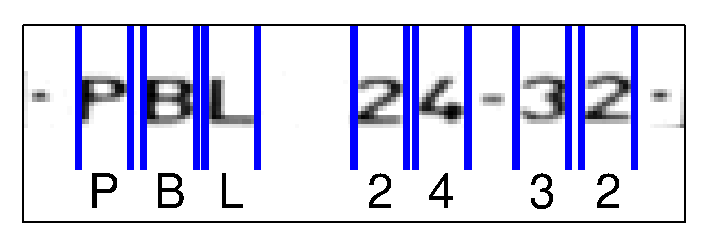
\includegraphics[width=0.3\textwidth]{matlab/lic_PBL2432.eps}}                
  \subfloat[\texttt{0} confused with \texttt{D}]{\label{fig:KLL72D8}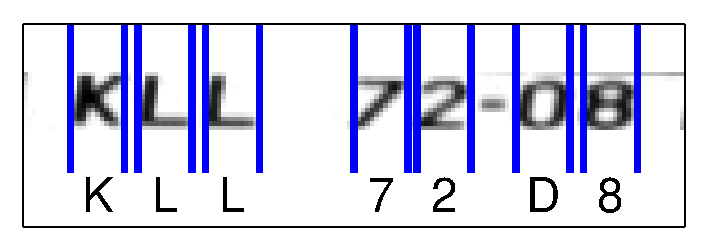
\includegraphics[width=0.3\textwidth]{matlab/lic_KLL72D8.eps}}
  \subfloat[\texttt{Z} confused with \texttt{2}]{\label{fig:mouse}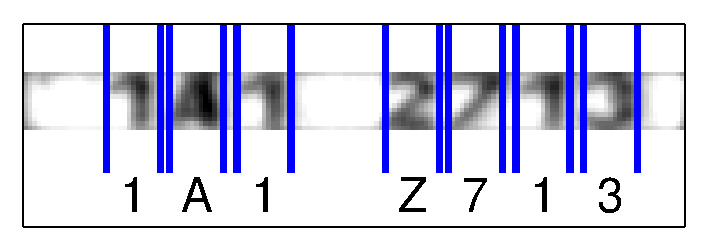
\includegraphics[width=0.3\textwidth]{matlab/lic_1A1Z713.eps}}
  \caption{Inferred vehicle ids from license plate images. Bottom
    line of text is the inferred string. Pairs of vertical blue bars
    are intervals of columns that were segmented as containing a
    character.}
  \label{fig:inferred-strings}
\end{figure}

\section{Evaluation}
Performance was measured on the test set \texttt{np-images-5000.mat}
consisting of 5000 annotated images of license plates.  Note that a
subset of the test set was used for training emissions distributions
too. Of interest is the quality of segmentation and accuracy of
license-string identification.  

Correct segmentation of a character is defined to be an interval of
columns given by the algorithm that intersects a region of the license
plate annotated as character within a specified tolerance. A proper
segmentation of the license plate is a sequence of correct character
segmentations for all annotated character regions.  Segmentation
errors occur if a character is nominated as white-space, a
\emph{missed detection}; or, conversely, white-space is nominated as a
character, a \emph{false alarm}.

The probability of detection $p_d$ is defined as the ratio of correctly
identified character regions to total number of annotated character regions
and the probability of false alarm $p_{fa}$ is identified as the number
of annotated white-space regions nominated as character regions to the
total number annotated white-space regions.

\begin{table}[ht]
\begin{center}
\begin{tabular}{|l|l|}
  \hline
  \multicolumn{2}{|c|}{Segmentation Performance} \\
  \hline
  $p_d$ & 71.9\% \\
  $p_{fa}$ & 7.60\% \\
  \hline
\end{tabular}
\caption{Calculated for \texttt{np-images-5000.mat}}
\end{center}
\end{table}

We require a metric on strings so that closeness of the inferred
\emph{vehicle-id} to the annotated \emph{vehicle-id} can be
measured. The Lenvenstein distance function $L$ between two strings is
defined as the minimum number of edits needed to transform one string
into the other, with the allowable edit operations being insertion,
deletion, or substitution of a single character. 

\begin{figure}[ht]
\begin{center}
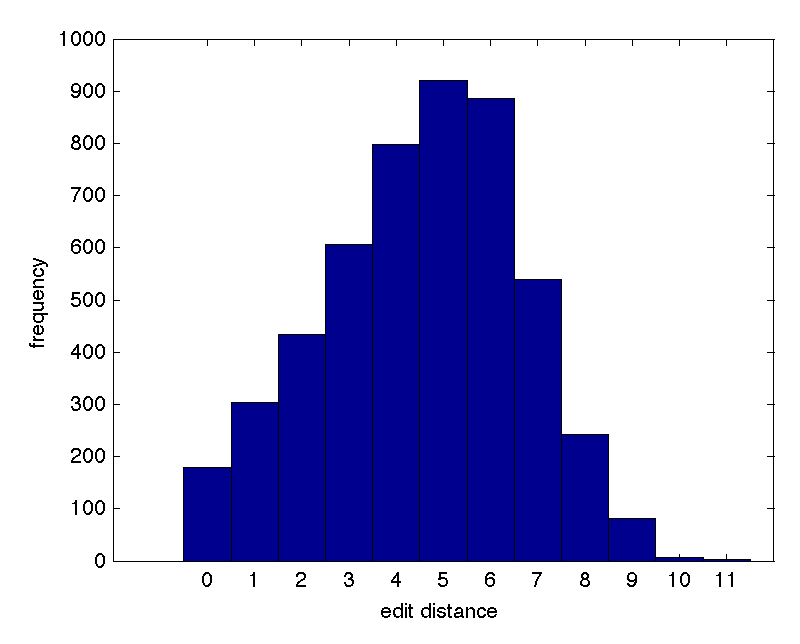
\includegraphics[width=0.75\linewidth]{matlab/hamming.eps}
\caption{ Frequency of edit distance over \texttt{np-images-5000.mat}  } 
\label{fig:editdistance}
\end{center}
\end{figure}

To determine the accuracy of the estimated \emph{vehicle-ids} for the
\texttt{np-images-5000.mat} test set, the expected Levenstein distance
between inferred id and ground-truth id is computed for all 5000
images.

\[ \text{accuracy} = \frac{\sum_{k \in \mathcal{U}}
  L(\hat{id}_k,id_k)}{8|\mathcal{U}|} \qquad U \text{ is test set
  \texttt{np-images-5000.mat} }  \]

\begin{table}[ht]
\begin{center}
\begin{tabular}{|l|l|}
  \hline
  \multicolumn{2}{|c|}{ID accuracy} \\
  \hline
  $accuracy$ & 36.5\% \\
  \hline
\end{tabular}
\caption{Calculated for \texttt{np-images-5000.mat}}
\end{center}
\end{table}

\section{Analysis and Suggested Improvements}
The performance, as suggested by the evaluation above, is not suitable
for operational use. The \textbf{HMM} used made many assumptions, so
there are many improvements to consider for better performance. As
expected, the \textbf{HMM} works best on clean exemplars from the data
set.

Most problematic is the overlap and large variance of the global
intensity models (see figure \ref{fig:distribution}) estimated during
training. Ideally, without de-focus blur and image artifacts, since the
image plate is high contrast, there should be two well-separated
distributions each with smaller variance. To account for image
corruption, more than two classes might be used to classify
intensities that are neither distinctly part of foreground or
background.

The transition model is too simple to account for cases caused by blur
where there is no apparent white space between characters, or the
character appears wider than our template. Furthermore, characters
such as \texttt{4} and \texttt{A}, and \texttt{0} and \texttt{D} look
like each other when blurred.

There was a significant variance of character width in the annotations
of \texttt{np-images-5000.mat}. This could arise from annotation error
or from errors in rectification. To
account for varying character widths in the test data, we allowed for 
non-zero transitions to the same glyph column.  A further improvement
would be to allow non-zero transitions between non-consecutive glyph
columns. 

Setting the transition probabilities manually was guided by some
simple observations of the training set. It is inevitable that we
missed some interactions in the data. Moving to supervised
learning to set the transition probabilities would likely capture
relations in the data that were overlooked. 

\end{document}

